% Options for packages loaded elsewhere
\PassOptionsToPackage{unicode}{hyperref}
\PassOptionsToPackage{hyphens}{url}
%
\documentclass[
  12 pt,
  a4paper,
]{article}
\usepackage{amsmath,amssymb}
\usepackage{setspace}
\usepackage{iftex}
\ifPDFTeX
  \usepackage[T1]{fontenc}
  \usepackage[utf8]{inputenc}
  \usepackage{textcomp} % provide euro and other symbols
\else % if luatex or xetex
  \usepackage{unicode-math} % this also loads fontspec
  \defaultfontfeatures{Scale=MatchLowercase}
  \defaultfontfeatures[\rmfamily]{Ligatures=TeX,Scale=1}
\fi
\usepackage{lmodern}
\ifPDFTeX\else
  % xetex/luatex font selection
  \setmainfont[]{Times New Roman}
\fi
% Use upquote if available, for straight quotes in verbatim environments
\IfFileExists{upquote.sty}{\usepackage{upquote}}{}
\IfFileExists{microtype.sty}{% use microtype if available
  \usepackage[]{microtype}
  \UseMicrotypeSet[protrusion]{basicmath} % disable protrusion for tt fonts
}{}
\makeatletter
\@ifundefined{KOMAClassName}{% if non-KOMA class
  \IfFileExists{parskip.sty}{%
    \usepackage{parskip}
  }{% else
    \setlength{\parindent}{0pt}
    \setlength{\parskip}{6pt plus 2pt minus 1pt}}
}{% if KOMA class
  \KOMAoptions{parskip=half}}
\makeatother
\usepackage{xcolor}
\usepackage[margin=1in]{geometry}
\usepackage{color}
\usepackage{fancyvrb}
\newcommand{\VerbBar}{|}
\newcommand{\VERB}{\Verb[commandchars=\\\{\}]}
\DefineVerbatimEnvironment{Highlighting}{Verbatim}{commandchars=\\\{\}}
% Add ',fontsize=\small' for more characters per line
\usepackage{framed}
\definecolor{shadecolor}{RGB}{248,248,248}
\newenvironment{Shaded}{\begin{snugshade}}{\end{snugshade}}
\newcommand{\AlertTok}[1]{\textcolor[rgb]{0.94,0.16,0.16}{#1}}
\newcommand{\AnnotationTok}[1]{\textcolor[rgb]{0.56,0.35,0.01}{\textbf{\textit{#1}}}}
\newcommand{\AttributeTok}[1]{\textcolor[rgb]{0.13,0.29,0.53}{#1}}
\newcommand{\BaseNTok}[1]{\textcolor[rgb]{0.00,0.00,0.81}{#1}}
\newcommand{\BuiltInTok}[1]{#1}
\newcommand{\CharTok}[1]{\textcolor[rgb]{0.31,0.60,0.02}{#1}}
\newcommand{\CommentTok}[1]{\textcolor[rgb]{0.56,0.35,0.01}{\textit{#1}}}
\newcommand{\CommentVarTok}[1]{\textcolor[rgb]{0.56,0.35,0.01}{\textbf{\textit{#1}}}}
\newcommand{\ConstantTok}[1]{\textcolor[rgb]{0.56,0.35,0.01}{#1}}
\newcommand{\ControlFlowTok}[1]{\textcolor[rgb]{0.13,0.29,0.53}{\textbf{#1}}}
\newcommand{\DataTypeTok}[1]{\textcolor[rgb]{0.13,0.29,0.53}{#1}}
\newcommand{\DecValTok}[1]{\textcolor[rgb]{0.00,0.00,0.81}{#1}}
\newcommand{\DocumentationTok}[1]{\textcolor[rgb]{0.56,0.35,0.01}{\textbf{\textit{#1}}}}
\newcommand{\ErrorTok}[1]{\textcolor[rgb]{0.64,0.00,0.00}{\textbf{#1}}}
\newcommand{\ExtensionTok}[1]{#1}
\newcommand{\FloatTok}[1]{\textcolor[rgb]{0.00,0.00,0.81}{#1}}
\newcommand{\FunctionTok}[1]{\textcolor[rgb]{0.13,0.29,0.53}{\textbf{#1}}}
\newcommand{\ImportTok}[1]{#1}
\newcommand{\InformationTok}[1]{\textcolor[rgb]{0.56,0.35,0.01}{\textbf{\textit{#1}}}}
\newcommand{\KeywordTok}[1]{\textcolor[rgb]{0.13,0.29,0.53}{\textbf{#1}}}
\newcommand{\NormalTok}[1]{#1}
\newcommand{\OperatorTok}[1]{\textcolor[rgb]{0.81,0.36,0.00}{\textbf{#1}}}
\newcommand{\OtherTok}[1]{\textcolor[rgb]{0.56,0.35,0.01}{#1}}
\newcommand{\PreprocessorTok}[1]{\textcolor[rgb]{0.56,0.35,0.01}{\textit{#1}}}
\newcommand{\RegionMarkerTok}[1]{#1}
\newcommand{\SpecialCharTok}[1]{\textcolor[rgb]{0.81,0.36,0.00}{\textbf{#1}}}
\newcommand{\SpecialStringTok}[1]{\textcolor[rgb]{0.31,0.60,0.02}{#1}}
\newcommand{\StringTok}[1]{\textcolor[rgb]{0.31,0.60,0.02}{#1}}
\newcommand{\VariableTok}[1]{\textcolor[rgb]{0.00,0.00,0.00}{#1}}
\newcommand{\VerbatimStringTok}[1]{\textcolor[rgb]{0.31,0.60,0.02}{#1}}
\newcommand{\WarningTok}[1]{\textcolor[rgb]{0.56,0.35,0.01}{\textbf{\textit{#1}}}}
\usepackage{longtable,booktabs,array}
\usepackage{calc} % for calculating minipage widths
% Correct order of tables after \paragraph or \subparagraph
\usepackage{etoolbox}
\makeatletter
\patchcmd\longtable{\par}{\if@noskipsec\mbox{}\fi\par}{}{}
\makeatother
% Allow footnotes in longtable head/foot
\IfFileExists{footnotehyper.sty}{\usepackage{footnotehyper}}{\usepackage{footnote}}
\makesavenoteenv{longtable}
\usepackage{graphicx}
\makeatletter
\def\maxwidth{\ifdim\Gin@nat@width>\linewidth\linewidth\else\Gin@nat@width\fi}
\def\maxheight{\ifdim\Gin@nat@height>\textheight\textheight\else\Gin@nat@height\fi}
\makeatother
% Scale images if necessary, so that they will not overflow the page
% margins by default, and it is still possible to overwrite the defaults
% using explicit options in \includegraphics[width, height, ...]{}
\setkeys{Gin}{width=\maxwidth,height=\maxheight,keepaspectratio}
% Set default figure placement to htbp
\makeatletter
\def\fps@figure{htbp}
\makeatother
\setlength{\emergencystretch}{3em} % prevent overfull lines
\providecommand{\tightlist}{%
  \setlength{\itemsep}{0pt}\setlength{\parskip}{0pt}}
\setcounter{secnumdepth}{-\maxdimen} % remove section numbering
\ifLuaTeX
\usepackage[bidi=basic]{babel}
\else
\usepackage[bidi=default]{babel}
\fi
\babelprovide[main,import]{spanish}
\ifPDFTeX
\else
\babelfont[spanish]{rm}{Times New Roman}
\fi
% get rid of language-specific shorthands (see #6817):
\let\LanguageShortHands\languageshorthands
\def\languageshorthands#1{}
\ifLuaTeX
  \usepackage{selnolig}  % disable illegal ligatures
\fi
\IfFileExists{bookmark.sty}{\usepackage{bookmark}}{\usepackage{hyperref}}
\IfFileExists{xurl.sty}{\usepackage{xurl}}{} % add URL line breaks if available
\urlstyle{same}
\hypersetup{
  pdfauthor={Tomàs Ferrandis Moscardó},
  pdflang={es-ES},
  hidelinks,
  pdfcreator={LaTeX via pandoc}}

\title{ANÁLISIS UNIVARIABLE SOBRE PROBABILIDAD DE VOTO SEGÚN BARÓMETRO
DEL CIS DE JULIO 2023\\
(ESTUDIO 3415)}
\usepackage{etoolbox}
\makeatletter
\providecommand{\subtitle}[1]{% add subtitle to \maketitle
  \apptocmd{\@title}{\par {\large #1 \par}}{}{}
}
\makeatother
\subtitle{Técnicas de Investigación en Ciencias Políticas-UBU.\\
Práctica 1. Apartado 4}
\author{Tomàs Ferrandis Moscardó}
\date{2023-03-22}

\begin{document}
\maketitle

{
\setcounter{tocdepth}{2}
\tableofcontents
}
\setstretch{1.5}
\newpage

\renewcommand\tablename{Tabla}

\hypertarget{introducciuxf3n}{%
\section{1 INTRODUCCIÓN}\label{introducciuxf3n}}

Esta actividad corresponde al apartado 4º de la Práctica 1 de Técnicas
de Investigación en Ciencia Política. Se trata de un \emph{análisis
univariado} sobre la variable PROBVOTO (pregunta P1) de la encuesta del
Barómetro de julio de 2023 (estudio 3415) vista en el apartado 3 y que
pregunta: \emph{Como Ud. sabe, el domingo 23 de julio se van a celebrar
elecciones generales en España. Para comenzar me gustaría que me dijera
cuál es la probabilidad de que Ud. vaya a votar. Para contestar utilice
una escala de 0 a 10 en la que el 0 significa ``con toda seguridad no
iría a votar'' y 10 ``con toda seguridad, iría a votar''}.

Por lo tanto se trata también de un \emph{análisis univariado},
descriptivo por tanto, aunque se le dará un tratamiento distinto.

Pese a ser un variable cualitativa ordinal, esta será manipulada como si
fuese una cuantitativa para obtener más información estadística. Se
trata de una práctica habitual en ciencias sociales que debe
justificarse en este caso porqué se observa se puede obtener más
información coherente.

Obviamente al tratarse de análisis univariado solo puede ser
descriptivo.

Como en la anterior actividad se incorpora el código R en los documentos
renderizados (HTML y PDF) opción \textbf{echo=TRUE} de los chunks. En
algunos chunks no interesa la impresión del resultado por lo que se
configuran con \textbf{results=`hide'}. Si se desea ver el resultado de
la ejecución correcta de alguno de estos chunks bastará con eliminar
esta parametrización en el fichero Rmd descargado (ver
\protect\hyperlink{id-github}{punto 7} ).

\begin{Shaded}
\begin{Highlighting}[]
\CommentTok{\# INSTALACIÓN (si no están instalados ) DE PAQUETES CON LAS LIBRERÍAS }
\CommentTok{\# NECESARIAS DE R (Se ocultan los mensajes de la instalación )}
\FunctionTok{suppressMessages}\NormalTok{(\{}
\ControlFlowTok{if}\NormalTok{ (}\SpecialCharTok{!}\FunctionTok{require}\NormalTok{(epiDisplay))\{}\FunctionTok{install.packages}\NormalTok{(}\StringTok{"epiDisplay"}\NormalTok{)\}}
\ControlFlowTok{if}\NormalTok{ (}\SpecialCharTok{!}\FunctionTok{require}\NormalTok{(e1071))\{}\FunctionTok{install.packages}\NormalTok{(}\StringTok{"e1071"}\NormalTok{)\}}
\ControlFlowTok{if}\NormalTok{ (}\SpecialCharTok{!}\FunctionTok{require}\NormalTok{(stats))\{}\FunctionTok{install.packages}\NormalTok{(}\StringTok{"stats"}\NormalTok{)\}}
\ControlFlowTok{if}\NormalTok{ (}\SpecialCharTok{!}\FunctionTok{require}\NormalTok{(tibble))\{}\FunctionTok{install.packages}\NormalTok{(}\StringTok{"tibble"}\NormalTok{)\}}
\ControlFlowTok{if}\NormalTok{ (}\SpecialCharTok{!}\FunctionTok{require}\NormalTok{(knitr))\{}\FunctionTok{install.packages}\NormalTok{(}\StringTok{"knitr"}\NormalTok{)\}}
\ControlFlowTok{if}\NormalTok{ (}\SpecialCharTok{!}\FunctionTok{require}\NormalTok{(haven))\{}\FunctionTok{install.packages}\NormalTok{(}\StringTok{"haven"}\NormalTok{)\}}
\NormalTok{\})}
\end{Highlighting}
\end{Shaded}

\newpage

\hypertarget{obtenciuxf3n-de-datos}{%
\section{2 OBTENCIÓN DE DATOS}\label{obtenciuxf3n-de-datos}}

\hypertarget{fichero-y-datos-en-abierto}{%
\subsection{2.1 Fichero y Datos en
Abierto}\label{fichero-y-datos-en-abierto}}

\begin{Shaded}
\begin{Highlighting}[]
\CommentTok{\# El fichero .sav lo debe estar en una subcarpeta DATOS}
\NormalTok{nombreFichero}\OtherTok{\textless{}{-}}\StringTok{"datosjulio2023.sav"}
\NormalTok{directorioTrabajo}\OtherTok{\textless{}{-}}\FunctionTok{getwd}\NormalTok{()}
\NormalTok{rutaFichero}\OtherTok{\textless{}{-}}\FunctionTok{paste}\NormalTok{(directorioTrabajo,}\StringTok{"DATOS"}\NormalTok{,nombreFichero,}\AttributeTok{sep=}\StringTok{"/"}\NormalTok{)}
\end{Highlighting}
\end{Shaded}

\hypertarget{creaciuxf3n-de-la-base-de-datos-data-frame}{%
\subsection{\texorpdfstring{2.2 Creación de la base de datos (\emph{data
frame})}{2.2 Creación de la base de datos (data frame)}}\label{creaciuxf3n-de-la-base-de-datos-data-frame}}

A partir del fichero de tipo \textbf{datosjulio2023.sav} descargado
desde el portal del CIS, se creará el \emph{data frame} de R. Esta será
la base de datos inicial con todos los datos de la encuesta.

\begin{Shaded}
\begin{Highlighting}[]
\NormalTok{df\_cisjulio}\OtherTok{\textless{}{-}}\FunctionTok{read\_sav}\NormalTok{(rutaFichero)}
\end{Highlighting}
\end{Shaded}

\begin{verbatim}
## Invalid date string (length=9): 25 038 23
\end{verbatim}

\hypertarget{consultar-el-cuestionario-y-el-diccionario-de-datos}{%
\subsection{2.3 Consultar el cuestionario y el diccionario de
datos}\label{consultar-el-cuestionario-y-el-diccionario-de-datos}}

Al margen de consultar el cuestionario del CIS, mediante funciones de R
se puede observar la variable para intentar deducir de qué tipo se
trata.

Algunas consultas posibles podrían ser:

\begin{enumerate}
\def\labelenumi{\arabic{enumi}.}
\tightlist
\item
  Consultar algunos casos y ver sus valores y etiquetas con
  \emph{head()} o \emph{tail()}
\item
  Agrupar todos los valores con la función \emph{unique}
\item
  Usar la función \emph{table} que devuelve el número de casos de cada
  valor.
\end{enumerate}

\begin{Shaded}
\begin{Highlighting}[]
\CommentTok{\# 1. Muestra los 5 últimos casos. Los valores y etiquetas}
\CommentTok{\# tail(df\_cisjulio$PROBVOTO,5) }
\CommentTok{\# 2. Obtiene los valores sin duplicados}
\CommentTok{\# unique(df\_cisjulio$PROBVOTO) }
\CommentTok{\# 3. table(df\_cisjulio$PROBVOTO) \# Nos da el total de casos que tiene }
            \CommentTok{\# cada valor}

\CommentTok{\# Uso de formato RMarkdown }
\FunctionTok{kable}\NormalTok{(}\FunctionTok{table}\NormalTok{(df\_cisjulio}\SpecialCharTok{$}\NormalTok{PROBVOTO),}\AttributeTok{column.width=}\FunctionTok{c}\NormalTok{(}\StringTok{"30\%"}\NormalTok{,}\StringTok{"70\%"}\NormalTok{),}
  \AttributeTok{col.names =} \FunctionTok{c}\NormalTok{(}\StringTok{"Valor"}\NormalTok{,}\StringTok{"Repeticiones"}\NormalTok{),}\AttributeTok{caption=}\StringTok{"Repeticiones de cada valor"}\NormalTok{)}
\end{Highlighting}
\end{Shaded}

\begin{longtable}[]{@{}lr@{}}
\caption{Repeticiones de cada valor}\tabularnewline
\toprule\noalign{}
Valor & Repeticiones \\
\midrule\noalign{}
\endfirsthead
\toprule\noalign{}
Valor & Repeticiones \\
\midrule\noalign{}
\endhead
\bottomrule\noalign{}
\endlastfoot
0 & 249 \\
1 & 35 \\
2 & 31 \\
3 & 32 \\
4 & 23 \\
5 & 183 \\
6 & 75 \\
7 & 117 \\
8 & 303 \\
9 & 574 \\
10 & 7145 \\
98 & 16 \\
99 & 15 \\
\end{longtable}

\newpage

\hypertarget{preparaciuxf3n-de-la-matriz-de-datos}{%
\section{3 PREPARACIÓN DE LA MATRIZ DE
DATOS}\label{preparaciuxf3n-de-la-matriz-de-datos}}

Una vez obtenida la matriz inicial de datos, se deberá limpiar y
simplificar esta base de datos inicial.

\hypertarget{limpieza-de-la-base-de-datos.}{%
\subsection{3.1 Limpieza de la base de
datos.}\label{limpieza-de-la-base-de-datos.}}

El data frame inicial contiene 141 columnas correspondientes a todas las
preguntas de la encuesta. Se puede prescindir del resto de columnas del
data frame innecesarias para nuestro análisis univariado.

\begin{Shaded}
\begin{Highlighting}[]
\NormalTok{df\_cisProbVoto}\OtherTok{\textless{}{-}}\NormalTok{df\_cisjulio [, }\StringTok{"PROBVOTO"}\NormalTok{]}
\CommentTok{\# ncol(df\_cisjulio) \# Para ver el número de columnas}
\end{Highlighting}
\end{Shaded}

Se ha reducido de 141 columna a 1 sola.

\hypertarget{recodificciuxf3n}{%
\subsection{3.2 Recodificción}\label{recodificciuxf3n}}

En este caso hay pocos valores válidos como es habitual en una variable
cualitativa (11 valores que son {[}0..10{]} ), no se va a agrupar
valores pero si se debe decidir qué valores no son válidos en la
estadística y excluirlos.

\hypertarget{se-duplica-la-columna}{%
\subsubsection{Se duplica la columna}\label{se-duplica-la-columna}}

Antes de modificar cualquier campo, se debe hacer un duplicado de este
(una nueva columna en el data frame) y trabajar sobre él.

\begin{Shaded}
\begin{Highlighting}[]
\CommentTok{\# Duplicación de columna}
\NormalTok{df\_cisProbVoto}\SpecialCharTok{$}\NormalTok{recPROBVOTO}\OtherTok{\textless{}{-}}\NormalTok{df\_cisProbVoto}\SpecialCharTok{$}\NormalTok{PROBVOTO }
\end{Highlighting}
\end{Shaded}

\hypertarget{valores-vuxe1lidos-y-valores-no-vuxe1lidos}{%
\subsubsection{Valores válidos y valores no
válidos}\label{valores-vuxe1lidos-y-valores-no-vuxe1lidos}}

Valores no válidos:

\begin{itemize}
\tightlist
\item
  98 N.S.
\item
  99 N.C.
\end{itemize}

Valores válidos:

\begin{itemize}
\tightlist
\item
  0,1,2,3,4,5,6,7,8,9,10
\end{itemize}

Los valores no válidos tienen un doble tratamiento:

\begin{itemize}
\tightlist
\item
  Valorar su importancia
\item
  Excluirlos de los cálculos
\end{itemize}

\hypertarget{importancia-de-los-valores-perdidos}{%
\paragraph{Importancia de los valores
perdidos}\label{importancia-de-los-valores-perdidos}}

Para valorar la incidencia o relevancia de los valores no válidos se
puede ver de qué porcentaje de casos sobre el total de la muestra se
trata.

Existen 31 de un total de 8798. Un porcentaje inferior a un 0.4 \% de
los casos y, por tanto, insignificante.

\hypertarget{asignar-na-para-excluir-en-el-anuxe1lisis}{%
\paragraph{Asignar NA para excluir en el
análisis}\label{asignar-na-para-excluir-en-el-anuxe1lisis}}

R permite excluir en sus funciones estadísticas los valores perdidos con
parametrizaciones al estilo \emph{MISSING=TRUE} o \emph{na.rm = TRUE}.
Para ello, previamente se tiene que asignar el valor NA a estos campos.

\begin{Shaded}
\begin{Highlighting}[]
\CommentTok{\# Los valores 98 y 99 (NS, NC ) pasan a NA}
\NormalTok{df\_cisProbVoto}\SpecialCharTok{$}\NormalTok{recPROBVOTO[df\_cisProbVoto}\SpecialCharTok{$}\NormalTok{recPROBVOTO}\SpecialCharTok{\textgreater{}=}\DecValTok{98}\NormalTok{]}\OtherTok{\textless{}{-}}\ConstantTok{NA}
\end{Highlighting}
\end{Shaded}

\newpage

\hypertarget{distribuciuxf3n-de-frecuencias}{%
\section{4. DISTRIBUCIÓN DE
FRECUENCIAS}\label{distribuciuxf3n-de-frecuencias}}

En este apartado se verá el uso de tablas de distribución de frecuencias
y gráficos. Ambos nos dan una idea de la frecuencia con que se repiten
los diferentes valores.

\hypertarget{gruxe1fico-de-barras}{%
\subsection{4.1 Gráfico de barras}\label{gruxe1fico-de-barras}}

\begin{Shaded}
\begin{Highlighting}[]
\NormalTok{tablaGrafico }\OtherTok{\textless{}{-}} \FunctionTok{tab1}\NormalTok{(df\_cisProbVoto}\SpecialCharTok{$}\NormalTok{recPROBVOTO, }\AttributeTok{cum.percent =} \ConstantTok{TRUE}\NormalTok{, }
                            \AttributeTok{bar.values =} \StringTok{"percent"}\NormalTok{, }\AttributeTok{missing =} \ConstantTok{FALSE}\NormalTok{,}
                                    \AttributeTok{xlab=}\StringTok{"\% probabilidad"}\NormalTok{, }\AttributeTok{decimal=}\DecValTok{1}\NormalTok{,}
                            \AttributeTok{main=}\StringTok{"Gráfico 1. Probabilidad de votar"}\NormalTok{)}
\end{Highlighting}
\end{Shaded}

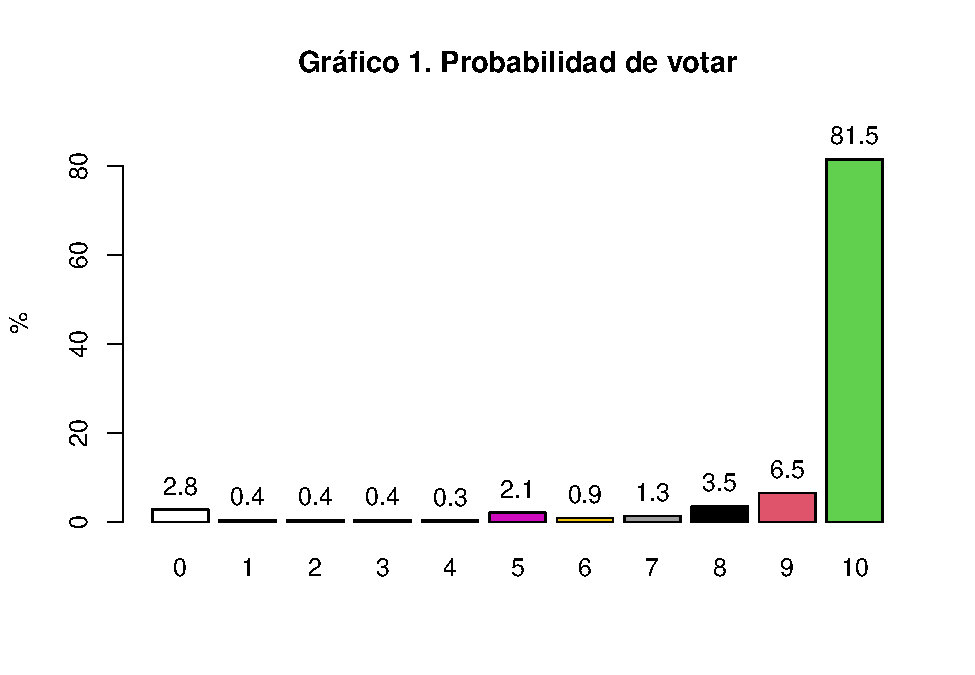
\includegraphics{probabilidadVoto_files/figure-latex/graficoBarras-1.pdf}

\hypertarget{tabla-de-frecuencias}{%
\subsection{4.2 Tabla de frecuencias}\label{tabla-de-frecuencias}}

En la tabla de frecuencias siguiente se muestra el total casos de la
muestra por cada valor, la frecuencia en que aparecen y la frecuencia
acumulada. Las frecuencias puede calcularse respecto al total de casos o
respecto al total de casos válidos. En este caso, como ya se ha apuntado
anteriormente, la diferencia es insignificante.

\begin{Shaded}
\begin{Highlighting}[]
\CommentTok{\# Mediante el atributo output.table se exporta una tabla}
\NormalTok{tabla}\OtherTok{\textless{}{-}}\NormalTok{tablaGrafico}\SpecialCharTok{$}\NormalTok{output.table}
\CommentTok{\#Para mejor la comprensión se puede cambiar los nombres de las columnas e }
\CommentTok{\# imprimir la tabla con Rmd}
\FunctionTok{colnames}\NormalTok{(tabla)}\OtherTok{\textless{}{-}}\FunctionTok{c}\NormalTok{(}\StringTok{"Frecuencia"}\NormalTok{,}\StringTok{"\%"}\NormalTok{,}\StringTok{"\%\_acumulado"}\NormalTok{, }\StringTok{"\%\_válido"}\NormalTok{,}
                                          \StringTok{"\%\_acumulado válido"}\NormalTok{)}

\FunctionTok{kable}\NormalTok{(tabla,}\AttributeTok{column.width =} \FunctionTok{c}\NormalTok{(}\StringTok{"10\%"}\NormalTok{,}\StringTok{"20\%"}\NormalTok{,}\StringTok{"20\%"}\NormalTok{,}\StringTok{"20\%"}\NormalTok{,}\StringTok{"20\%"}\NormalTok{),}
                \AttributeTok{caption=}\StringTok{"Tabla de distribución de frecuencias"}\NormalTok{) }
\end{Highlighting}
\end{Shaded}

\begin{longtable}[]{@{}lrrrrr@{}}
\caption{Tabla de distribución de frecuencias}\tabularnewline
\toprule\noalign{}
& Frecuencia & \% & \%\_acumulado & \%\_válido & \%\_acumulado válido \\
\midrule\noalign{}
\endfirsthead
\toprule\noalign{}
& Frecuencia & \% & \%\_acumulado & \%\_válido & \%\_acumulado válido \\
\midrule\noalign{}
\endhead
\bottomrule\noalign{}
\endlastfoot
0 & 249 & 2.8 & 2.8 & 2.8 & 2.8 \\
1 & 35 & 0.4 & 3.2 & 0.4 & 3.2 \\
2 & 31 & 0.4 & 3.6 & 0.4 & 3.6 \\
3 & 32 & 0.4 & 3.9 & 0.4 & 4.0 \\
4 & 23 & 0.3 & 4.2 & 0.3 & 4.2 \\
5 & 183 & 2.1 & 6.3 & 2.1 & 6.3 \\
6 & 75 & 0.9 & 7.1 & 0.9 & 7.2 \\
7 & 117 & 1.3 & 8.5 & 1.3 & 8.5 \\
8 & 303 & 3.4 & 11.9 & 3.5 & 12.0 \\
9 & 574 & 6.5 & 18.4 & 6.5 & 18.5 \\
10 & 7145 & 81.2 & 99.6 & 81.5 & 100.0 \\
NA & 31 & 0.4 & 100.0 & 0.0 & 100.0 \\
Total & 8798 & 100.0 & 100.0 & 100.0 & 100.0 \\
\end{longtable}

\begin{Shaded}
\begin{Highlighting}[]
\CommentTok{\# print(tabla)  \# En R estrictamente (no Rmd)}

\CommentTok{\# Para calcular solo las frecuencias de cada valor directamente:}
\CommentTok{\# round(prop.table(table(df\_cisProbVoto$recPROBVOTO, useNA="no"))*100,1)}
\end{Highlighting}
\end{Shaded}

\newpage

\hypertarget{tratamiento-como-variable-cuantitativa}{%
\section{5 TRATAMIENTO COMO VARIABLE
CUANTITATIVA}\label{tratamiento-como-variable-cuantitativa}}

Aunque la ``probabilidad de votar'' en este cuestionario se trata de una
variable \emph{cualitativa ordinal}, se podría asumir que los valores
válidos {[}0..10{]} representan una magnitud que admite operaciones
aritméticas y darle un tratamiento de \emph{variable cuantitativa}. En
este contexto podría entenderse como de variable \emph{razón} si se
asume el valor 0 como la ausencia absoluta de intención de ir a votar
(cero absoluto). No obstante se trata de una interpretación que no debe
sacarse del contexto de este análisis concreto.

Este planteamiento, excepcional, se justifica por la necesidad de
obtener los valores de las \emph{medidas de tendencia central} más allá
de la \emph{moda}.

\hypertarget{medidas-de-tendencia-central}{%
\subsection{5.1 Medidas de tendencia
central}\label{medidas-de-tendencia-central}}

\hypertarget{funciuxf3n-summary}{%
\subsubsection{\texorpdfstring{Función
\emph{summary}}{Función summary}}\label{funciuxf3n-summary}}

Esta función nos aporta las medidas de posición central (moda, media y
mediana) y las de posición no central (valores extremos y cuartiles). El
segundo cuartil equivale a la mediana.

\begin{Shaded}
\begin{Highlighting}[]
\FunctionTok{summary}\NormalTok{(df\_cisProbVoto}\SpecialCharTok{$}\NormalTok{recPROBVOTO,}\AttributeTok{digits=}\DecValTok{2}\NormalTok{)  }\CommentTok{\#Digits: dígitos significativos}
\end{Highlighting}
\end{Shaded}

\begin{verbatim}
##    Min. 1st Qu.  Median    Mean 3rd Qu.    Max.    NA's 
##     0.0    10.0    10.0     9.3    10.0    10.0      31
\end{verbatim}

\hypertarget{media-mediana-y-moda}{%
\subsubsection{Media, Mediana y Moda}\label{media-mediana-y-moda}}

Estas medidas de posición central se pueden obtener mediante funciones
de R con posibilidad de parametrizar su cálculo (borrar NA, número de
decimales\ldots) y evidentemente guardar su valor de retorno en una
variable para su posterior uso.

\begin{itemize}
\tightlist
\item
  La opción \emph{na.rm = TRUE} indica que no se debe considerar los
  valores no validos
\item
  El valor obtenido se puede redondear con la función \emph{round}. En
  ciencias sociales lo habitual es 1 decimal
\end{itemize}

\hypertarget{media}{%
\paragraph{Media}\label{media}}

Promedio aritmético de todos los valores de la muestra.

\begin{Shaded}
\begin{Highlighting}[]
\NormalTok{media}\OtherTok{\textless{}{-}}\FunctionTok{round}\NormalTok{(}\FunctionTok{mean}\NormalTok{(df\_cisProbVoto}\SpecialCharTok{$}\NormalTok{recPROBVOTO, }\AttributeTok{na.rm =} \ConstantTok{TRUE}\NormalTok{),}\DecValTok{1}\NormalTok{)}
\end{Highlighting}
\end{Shaded}

\hypertarget{mediana}{%
\paragraph{Mediana}\label{mediana}}

Valor de la muestra que divide la muestra en dos mitades o grupos con
igual cantidad de casos, siendo uno de los grupos el formado por casos
con un valor superior y el otro grupo el formado por los casos con valor
inferior.

\begin{Shaded}
\begin{Highlighting}[]
\NormalTok{mediana}\OtherTok{\textless{}{-}}\FunctionTok{median}\NormalTok{(df\_cisProbVoto}\SpecialCharTok{$}\NormalTok{recPROBVOTO, }\AttributeTok{na.rm =} \ConstantTok{TRUE}\NormalTok{,}\DecValTok{1}\NormalTok{)}
\end{Highlighting}
\end{Shaded}

\hypertarget{moda}{%
\paragraph{Moda}\label{moda}}

La moda es el valor de la muestra que más se repite. Como ya se vio en
la actividad anterior de esta práctica, en R no existe una función que
devuelva la moda directamente similar a las vistas para mediana
\emph{median()} y para la media \emph{mean()}.

Se debe usar una diseñada expresamente que, una vez definida, se puede
llamar de igual manera que a las librerías predefinidas de R e
incorporadas con la instalación de los paquetes.

\emph{Función moda}

\begin{Shaded}
\begin{Highlighting}[]
\CommentTok{\#declaración y desarrollo de la función de usuario}
\NormalTok{moda}\OtherTok{\textless{}{-}} \ControlFlowTok{function}\NormalTok{(v) \{}
\NormalTok{uniqv }\OtherTok{\textless{}{-}} \FunctionTok{unique}\NormalTok{(v)}
\NormalTok{uniqv[}\FunctionTok{which.max}\NormalTok{(}\FunctionTok{tabulate}\NormalTok{(}\FunctionTok{match}\NormalTok{(v, uniqv)))]}
\NormalTok{\}}
\end{Highlighting}
\end{Shaded}

\begin{Shaded}
\begin{Highlighting}[]
\CommentTok{\#Se llama a la función previamente desarrollada}
\NormalTok{moda}\OtherTok{\textless{}{-}}\FunctionTok{moda}\NormalTok{(df\_cisProbVoto}\SpecialCharTok{$}\NormalTok{recPROBVOTO) }
\end{Highlighting}
\end{Shaded}

\textbf{Resumen de valores de posición central}

\begin{itemize}
\tightlist
\item
  La Media es 9.3
\item
  La Mediana es 10
\item
  La Moda es 10
\end{itemize}

\textbf{Conclusiones}

La \emph{media aritmética}: 9.3 está muy influida por la altísima
frecuencia de los valores más altos, sobretodo del máximo (10). Pese a
que la \emph{Mediana} nos de como resultado 10, el total de casos con
valor inferior no llega a ser el 50\%.

La moda sin duda es el valor 10 como ya se podía deducir a partir del
porcentaje reflejado en la tabla de frecuencia.

\hypertarget{comparaciuxf3n-entre-moda-media-y-mediana.}{%
\subsection{5.2 Comparación entre Moda, Media y
Mediana.}\label{comparaciuxf3n-entre-moda-media-y-mediana.}}

\textbf{Histograma}

El histograma mostrará una asimetría positiva (sesgo a la izquierda)
donde la media y a moda coinciden y la media es el valor más bajo

\textbf{X\textless Me=Mo}

\begin{Shaded}
\begin{Highlighting}[]
\CommentTok{\# Eliminar filas con NA}
\NormalTok{df\_cisProbVotoSinNA }\OtherTok{\textless{}{-}}\NormalTok{ df\_cisProbVoto[}\FunctionTok{complete.cases}\NormalTok{(}
\NormalTok{                                      df\_cisProbVoto}\SpecialCharTok{$}\NormalTok{recPROBVOTO), ]}

\FunctionTok{hist}\NormalTok{(df\_cisProbVoto}\SpecialCharTok{$}\NormalTok{recPROBVOTO, }\AttributeTok{col =} \StringTok{"lightblue"}\NormalTok{, }
                                          \AttributeTok{xlab =} \StringTok{"Probabilidad de voto"}\NormalTok{, }
                                                     \AttributeTok{ylab =} \StringTok{"Frecuencia"}\NormalTok{,}
              \AttributeTok{main =} \StringTok{"Gráfico 2. Histograma de la probabilidad de votar"}\NormalTok{)}

\FunctionTok{lines}\NormalTok{(}\FunctionTok{density}\NormalTok{(df\_cisProbVotoSinNA}\SpecialCharTok{$}\NormalTok{recPROBVOTO), }\AttributeTok{col =} \StringTok{"red"}\NormalTok{, }\AttributeTok{lwd =} \DecValTok{1}\NormalTok{)}
\end{Highlighting}
\end{Shaded}

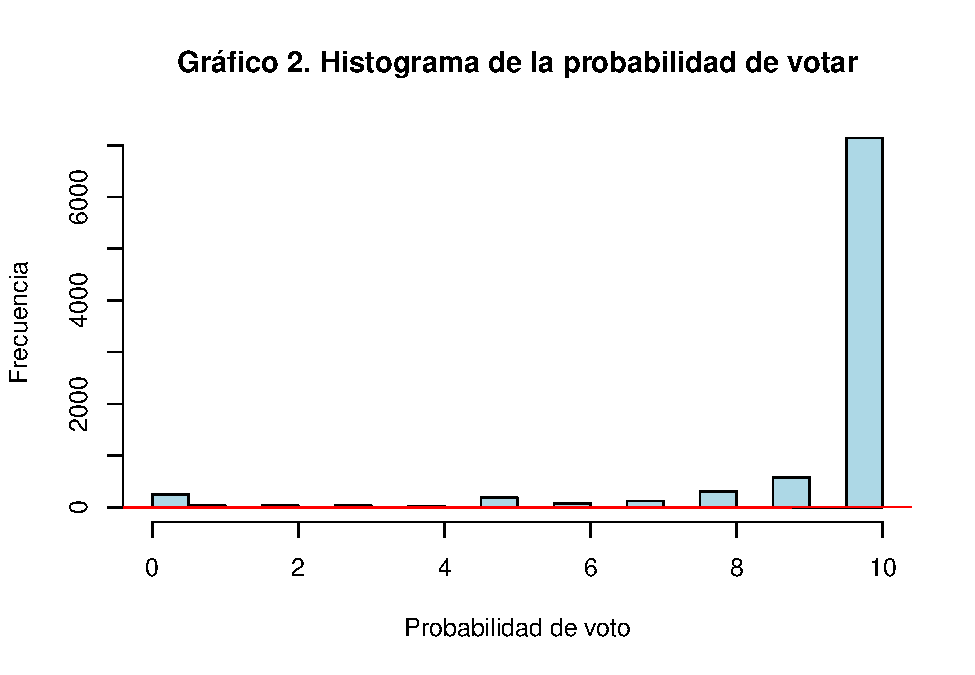
\includegraphics{probabilidadVoto_files/figure-latex/histograma-1.pdf}
\#\#\# Conclusión sobre las medidas de posición central

Viendo el sesgo (a la derecha) se entiende que la mediana tenga un valor
mayor que la moda y menor que la Media. La mediana debería ser una
medida de posición central mejor que la media ya que esta quedaría
distorsionada por los extremos. La moda viene definida por la repetición
de un valor. En nuestro caso, en cambio, la mediana coincide con la
Moda.

\hypertarget{medidas-de-posiciuxf3n-no-central}{%
\subsection{5.3 Medidas de posición no
central}\label{medidas-de-posiciuxf3n-no-central}}

\hypertarget{valores-extremos-muxe1ximo-y-muxednimo}{%
\subsubsection{Valores extremos: Máximo y
Mínimo}\label{valores-extremos-muxe1ximo-y-muxednimo}}

\begin{Shaded}
\begin{Highlighting}[]
\CommentTok{\# Se guardan en variables los retorno de las funciones predefinidas de R}
\CommentTok{\# así se pueden leer desde le MD}
\NormalTok{maximo}\OtherTok{\textless{}{-}}\FunctionTok{max}\NormalTok{(df\_cisProbVoto}\SpecialCharTok{$}\NormalTok{recPROBVOTO, }\AttributeTok{na.rm =} \ConstantTok{TRUE}\NormalTok{)}
\NormalTok{minimo}\OtherTok{\textless{}{-}}\FunctionTok{min}\NormalTok{(df\_cisProbVoto}\SpecialCharTok{$}\NormalTok{recPROBVOTO, }\AttributeTok{na.rm =} \ConstantTok{TRUE}\NormalTok{)}
\end{Highlighting}
\end{Shaded}

Los valores extremos son:

\begin{itemize}
\tightlist
\item
  El valor MÁXIMO es: 10
\item
  El valor MÍNIMO es: 0
\end{itemize}

Al tratarse de una pregunta cerrada con una ordenación entre las
respuestas (variable cualitativa ordinal), estos valores indican el par
de respuestas más dispares entre si de nuestra muestra. La coincidencia
de máximo y mínimo con las opciones más extremas posibles significa
simplemente que en nuestra muestra ha habido, al menos, un caso (persona
encuestada) que ha elegido un extremo.

\hypertarget{cuartiles-y-percentiles}{%
\subsubsection{Cuartiles y percentiles}\label{cuartiles-y-percentiles}}

En una distribución de valores de una muestra tan sesgada, un cuartil no
da demasiada información. La inmensa mayoría de valores son 10 y el
resto son tratados como valores atípicos (1,5 veces la caja).

\begin{Shaded}
\begin{Highlighting}[]
\CommentTok{\# Crear el diagrama de caja}
\FunctionTok{boxplot}\NormalTok{(df\_cisProbVotoSinNA}\SpecialCharTok{$}\NormalTok{recPROBVOTO, }
        \AttributeTok{main =} \StringTok{"Gráfico 3. Cuartiles probabilidad de votar"}\NormalTok{,}
        \AttributeTok{ylab =} \StringTok{"Valores de 0 a 10"}\NormalTok{, }
        \AttributeTok{col =} \StringTok{"lightblue"}\NormalTok{)}

\CommentTok{\# Calcular los cuartiles}
\NormalTok{cuartiles }\OtherTok{\textless{}{-}} \FunctionTok{quantile}\NormalTok{(df\_cisProbVotoSinNA}\SpecialCharTok{$}\NormalTok{recPROBVOTO, }
                            \AttributeTok{probs =} \FunctionTok{c}\NormalTok{(}\FloatTok{0.25}\NormalTok{, }\FloatTok{0.5}\NormalTok{, }\FloatTok{0.75}\NormalTok{))}

\CommentTok{\# Agregar las líneas de los los cuartiles}
\FunctionTok{abline}\NormalTok{(}\AttributeTok{h =}\NormalTok{ cuartiles, }\AttributeTok{col =} \FunctionTok{c}\NormalTok{(}\StringTok{"red"}\NormalTok{, }\StringTok{"green"}\NormalTok{, }\StringTok{"blue"}\NormalTok{))}
\end{Highlighting}
\end{Shaded}

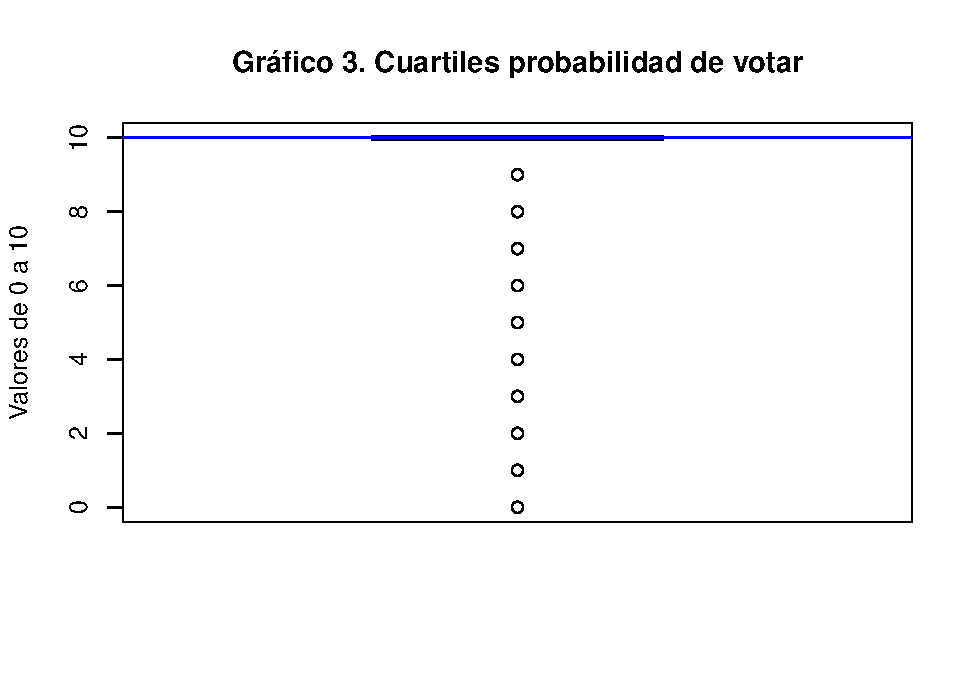
\includegraphics{probabilidadVoto_files/figure-latex/cuartiles-1.pdf}

Se puede usar los percentiles para analizar mejor la información.

\begin{Shaded}
\begin{Highlighting}[]
\NormalTok{percentiles}\OtherTok{\textless{}{-}}\FunctionTok{quantile}\NormalTok{(df\_cisProbVotoSinNA, }\FunctionTok{c}\NormalTok{(.}\DecValTok{10}\NormalTok{,.}\DecValTok{20}\NormalTok{,.}\DecValTok{30}\NormalTok{,.}\DecValTok{40}\NormalTok{,.}\DecValTok{50}\NormalTok{,.}\DecValTok{60}\NormalTok{,.}\DecValTok{70}\NormalTok{,}
\NormalTok{                                                  .}\DecValTok{80}\NormalTok{,.}\DecValTok{90}\NormalTok{), }\AttributeTok{na.rm =} \ConstantTok{TRUE}\NormalTok{)}
\FunctionTok{boxplot}\NormalTok{(df\_cisProbVotoSinNA}\SpecialCharTok{$}\NormalTok{recPROBVOTO, }
                    \AttributeTok{main =} \StringTok{"Gráfico 4. Percentiles probabilidad de votar"}\NormalTok{,}
                            \AttributeTok{ylab =} \StringTok{"Valores de 0 a 10"}\NormalTok{, }\AttributeTok{col =} \StringTok{"lightblue"}\NormalTok{)}

\CommentTok{\# Agregar las líneas de los los cuartiles}
\FunctionTok{abline}\NormalTok{(}\AttributeTok{h =}\NormalTok{ percentiles, }\AttributeTok{col =} \StringTok{"red"}\NormalTok{)}
\end{Highlighting}
\end{Shaded}

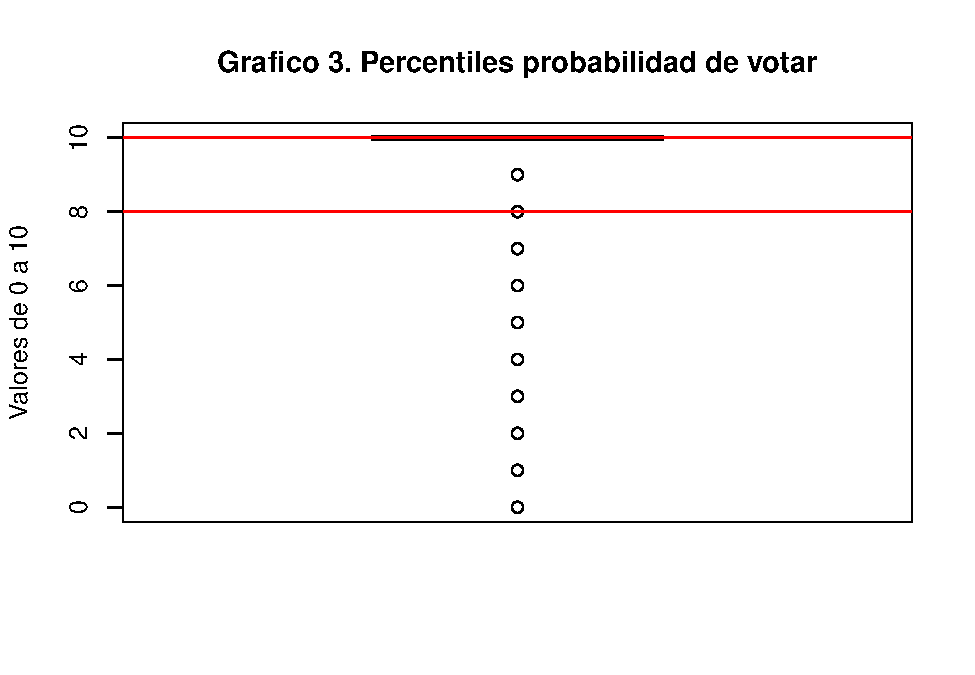
\includegraphics{probabilidadVoto_files/figure-latex/percentiles0-1.pdf}

\begin{Shaded}
\begin{Highlighting}[]
\NormalTok{percentiles}\OtherTok{\textless{}{-}}\FunctionTok{quantile}\NormalTok{(df\_cisProbVotoSinNA, }\FunctionTok{c}\NormalTok{(.}\DecValTok{02}\NormalTok{,.}\DecValTok{03}\NormalTok{,.}\DecValTok{04}\NormalTok{,.}\DecValTok{05}\NormalTok{,.}\DecValTok{06}\NormalTok{,.}\DecValTok{07}\NormalTok{,.}\DecValTok{08}\NormalTok{,}
\NormalTok{                  .}\DecValTok{09}\NormalTok{,.}\DecValTok{10}\NormalTok{,.}\DecValTok{20}\NormalTok{,.}\DecValTok{30}\NormalTok{,.}\DecValTok{40}\NormalTok{,.}\DecValTok{50}\NormalTok{,.}\DecValTok{60}\NormalTok{,.}\DecValTok{70}\NormalTok{,.}\DecValTok{80}\NormalTok{,.}\DecValTok{90}\NormalTok{), }\AttributeTok{na.rm =} \ConstantTok{TRUE}\NormalTok{)}
\FunctionTok{boxplot}\NormalTok{(df\_cisProbVotoSinNA}\SpecialCharTok{$}\NormalTok{recPROBVOTO, }
                    \AttributeTok{main =} \StringTok{"Gráfico 5. Percentiles probabilidad de votar"}\NormalTok{,}
                            \AttributeTok{ylab =} \StringTok{"Valores de 0 a 10"}\NormalTok{, }\AttributeTok{col =} \StringTok{"lightblue"}\NormalTok{)}

\CommentTok{\# Agregar las líneas de los los cuartiles}
\FunctionTok{abline}\NormalTok{(}\AttributeTok{h =}\NormalTok{ percentiles, }\AttributeTok{col =} \FunctionTok{c}\NormalTok{(}\StringTok{"red"}\NormalTok{, }\StringTok{"green"}\NormalTok{, }\StringTok{"blue"}\NormalTok{,}\StringTok{"red"}\NormalTok{, }\StringTok{"green"}\NormalTok{,}
                                \StringTok{"blue"}\NormalTok{,}\StringTok{"red"}\NormalTok{, }\StringTok{"green"}\NormalTok{,}\StringTok{"blue"}\NormalTok{,}\StringTok{"red"}\NormalTok{,}
                                \StringTok{"green"}\NormalTok{, }\StringTok{"blue"}\NormalTok{,}\StringTok{"red"}\NormalTok{, }\StringTok{"green"}\NormalTok{, }
                                \StringTok{"blue"}\NormalTok{,}\StringTok{"red"}\NormalTok{, }\StringTok{"green"}\NormalTok{, }\StringTok{"blue"}\NormalTok{))}
\end{Highlighting}
\end{Shaded}

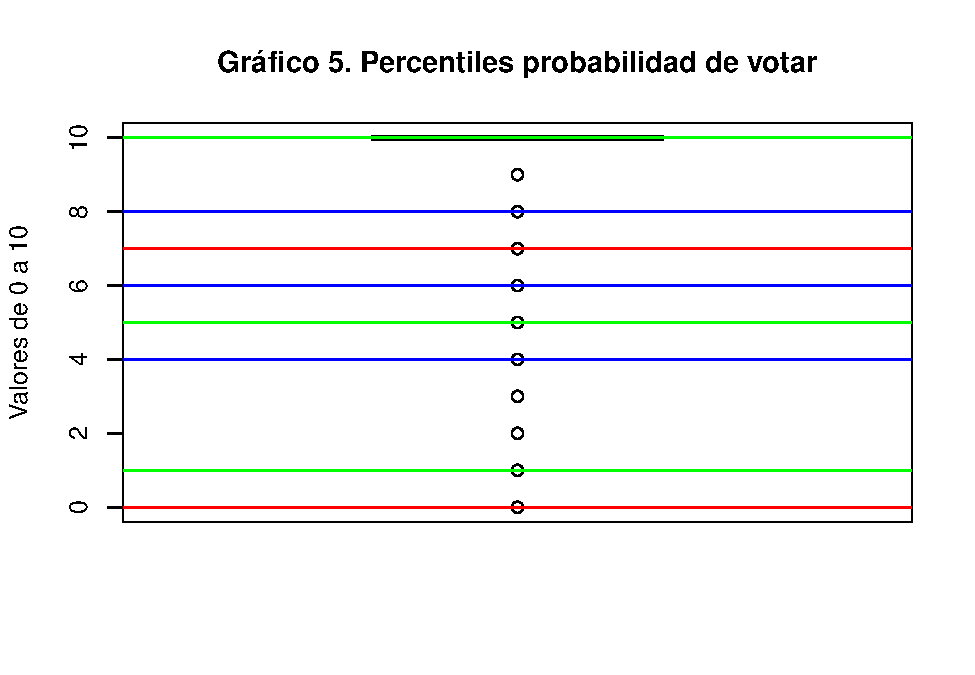
\includegraphics{probabilidadVoto_files/figure-latex/percentiles-1.pdf}
\emph{Conclusión:}

Solo un porcentaje inferior al 9\% de la muestra ha respondido un valor
inferior al `8'. Un hecho que se puede apreciar también en la columna de
\emph{frecuencias acumuladas} (Tabla de frecuencia) donde el valor 8
acumula el 8,5\%.

\hypertarget{medidas-de-dispersiuxf3n}{%
\subsection{5.4 Medidas de dispersión}\label{medidas-de-dispersiuxf3n}}

Se procederá a obtener las medidas de variabilidad o dispersión que
informan del comportamiento de la variable y complementan la información
sobre la centralidad.

\hypertarget{varianza-o-desviaciuxf3n-tuxedpica}{%
\subsubsection{Varianza o desviación
típica}\label{varianza-o-desviaciuxf3n-tuxedpica}}

\begin{Shaded}
\begin{Highlighting}[]
\CommentTok{\# na.rm = TRUE. Si en el data frame existen valores perdidos.}
\NormalTok{varianza}\OtherTok{\textless{}{-}}\FunctionTok{var}\NormalTok{(df\_cisProbVoto}\SpecialCharTok{$}\NormalTok{recPROBVOTO,}\AttributeTok{na.rm =} \ConstantTok{TRUE}\NormalTok{)}
\end{Highlighting}
\end{Shaded}

La desviación típica es: 4.2

\hypertarget{desviaciuxf3n-estuxe1ndar}{%
\subsubsection{Desviación Estándar}\label{desviaciuxf3n-estuxe1ndar}}

\begin{Shaded}
\begin{Highlighting}[]
\CommentTok{\# na.rm = TRUE. Si en el data frame existen valores perdidos.}
\NormalTok{desviacionEstandar}\OtherTok{\textless{}{-}}\FunctionTok{sd}\NormalTok{(df\_cisProbVoto}\SpecialCharTok{$}\NormalTok{recPROBVOTO, }\AttributeTok{na.rm =} \ConstantTok{TRUE}\NormalTok{)}
\end{Highlighting}
\end{Shaded}

La desviación estándar es: 2

\hypertarget{rango-intercuatuxedlico}{%
\subsubsection{Rango intercuatílico}\label{rango-intercuatuxedlico}}

\begin{Shaded}
\begin{Highlighting}[]
\CommentTok{\# na.rm = TRUE. Si en el data frame existen valores perdidos.}
\NormalTok{iqr}\OtherTok{\textless{}{-}}\FunctionTok{IQR}\NormalTok{(df\_cisProbVoto}\SpecialCharTok{$}\NormalTok{recPROBVOTO, }\AttributeTok{na.rm =} \ConstantTok{TRUE}\NormalTok{)}
\end{Highlighting}
\end{Shaded}

El rango intercuartílico es 0

\hypertarget{curtosis}{%
\subsubsection{Curtosis}\label{curtosis}}

El coeficiente de curtosis indica el nivel de apuntamiento achatamiento
que presenta una distribución de valores. Solo tiene sentidos en
distribuciones unimodales y simétricas. No es este nuestro caso.

\begin{Shaded}
\begin{Highlighting}[]
\CommentTok{\# na.rm = TRUE. Si en el data frame existen valores perdidos.}
\NormalTok{coeficienteKurtosis}\OtherTok{\textless{}{-}}\FunctionTok{kurtosis}\NormalTok{(df\_cisProbVoto}\SpecialCharTok{$}\NormalTok{recPROBVOTO, }\AttributeTok{na.rm =} \ConstantTok{TRUE}\NormalTok{)}
\end{Highlighting}
\end{Shaded}

El coeficiente de curtosis es: 11.9497589

\hypertarget{coeficiente-de-asimetruxeda}{%
\subsubsection{Coeficiente de
Asimetría}\label{coeficiente-de-asimetruxeda}}

\begin{Shaded}
\begin{Highlighting}[]
\NormalTok{coeficienteAsimetria}\OtherTok{\textless{}{-}}\FunctionTok{skewness}\NormalTok{(df\_cisProbVoto}\SpecialCharTok{$}\NormalTok{recPROBVOTO, }\AttributeTok{na.rm =} \ConstantTok{TRUE}\NormalTok{)}
\end{Highlighting}
\end{Shaded}

El coeficiente de asimetría es: -3.5101093

\hypertarget{grafico-de-densidad}{%
\subsubsection{Grafico de densidad}\label{grafico-de-densidad}}

\begin{Shaded}
\begin{Highlighting}[]
\FunctionTok{plot}\NormalTok{(df\_cisProbVoto}\SpecialCharTok{$}\NormalTok{recPROBVOTO,}\AttributeTok{main=}\StringTok{"Gráfico 6. Gráfico de densidad"}
\NormalTok{                        ,}\AttributeTok{xlab=}\StringTok{"Casos"}\NormalTok{, }\AttributeTok{ylab =} \StringTok{"Probabilidad de voto"}\NormalTok{)}
\end{Highlighting}
\end{Shaded}

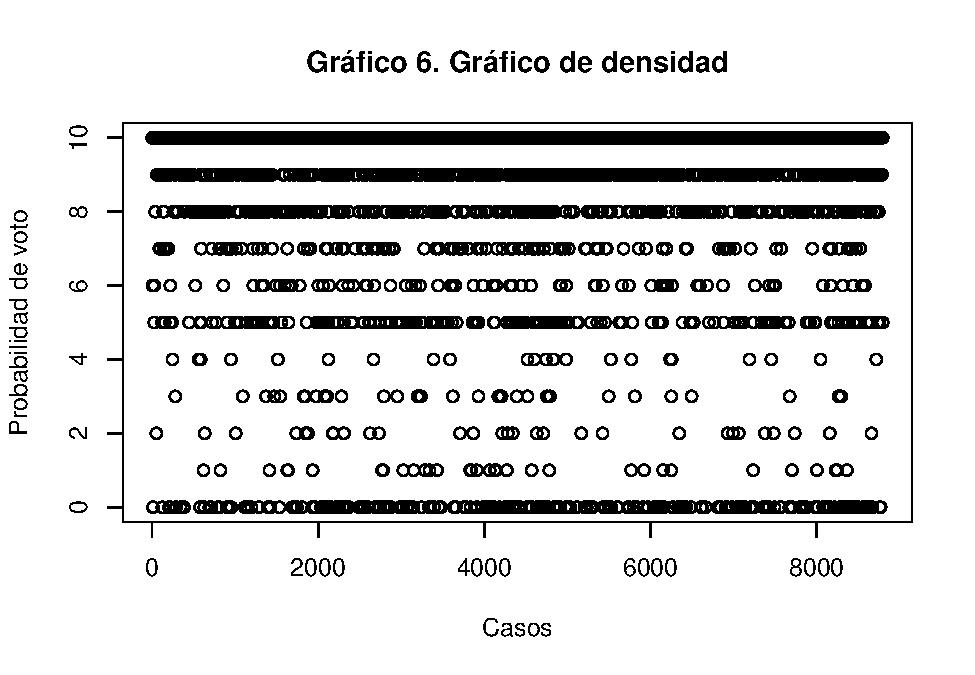
\includegraphics{probabilidadVoto_files/figure-latex/graficoDensidad-1.pdf}

\newpage

\hypertarget{resumen-valores}{%
\section{6 RESUMEN VALORES}\label{resumen-valores}}

Tabla 3: Resumen de valores de las mediciones

\begin{longtable}[]{@{}lr@{}}
\toprule\noalign{}
\textbf{Medición} & \textbf{Valor} \\
\midrule\noalign{}
\endhead
\bottomrule\noalign{}
\endlastfoot
\textbf{POSICIÓN CENTRAL (Medidas de tendencia central)} & \\
MODA & 10 \\
MEDIANA & 10 \\
MEDIA & 9.3 \\
\textbf{POSICIÓN (Medidas de posición no central)} & \\
MÁXIMO & 10 \\
MÍNIMO & 0 \\
PERCENTIL 25 & 10 \\
PERCENTIL 50 & 10 \\
PERCENTIL 75 & 10 \\
\textbf{MEDIDAS DE DISPERSIÓN} & \\
RANGO & 10 \\
RANGO INTERCUARTIL & 0 \\
DESVIACIÓN TÍPICA & 4.2 \\
DESVIACIÓN TÍPICA & 2 \\
\textbf{MEDIDAS DE FORMA} & \\
COEFICIENTE DE ASIMETRÍA & -3.5 \\
COEFICIENTE DE KURTOSIS & 12 \\
\end{longtable}

\newpage

\hypertarget{id-github}{%
\section{7 EJECUCIÓN DEL Rmd Y REPOSITORIO DE
FICHEROS}\label{id-github}}

Para la ejecución del código R, está disponible el fichero ejecutable
Rmd y el fichero de datos \emph{sav} en el repositorio GitHub. En el
mismo repositorio se encuentra este PDF y un fichero HTML renderizados a
partir del Rmd.

El fichero \textbf{datosjulio2023.sav} debe ubicarse en una subcarpeta
del directorio de trabajo con nombre \emph{DATA}.

\begin{longtable}[]{@{}
  >{\centering\arraybackslash}p{(\columnwidth - 4\tabcolsep) * \real{0.2500}}
  >{\raggedright\arraybackslash}p{(\columnwidth - 4\tabcolsep) * \real{0.3500}}
  >{\raggedright\arraybackslash}p{(\columnwidth - 4\tabcolsep) * \real{0.4000}}@{}}
\toprule\noalign{}
\begin{minipage}[b]{\linewidth}\centering

\includegraphics[width=0.1\textwidth,height=\textheight]{../../recursos/iconohyperlink.jpg}
\end{minipage} & \begin{minipage}[b]{\linewidth}\raggedright
\end{minipage} & \begin{minipage}[b]{\linewidth}\raggedright
Enlace a GitHub
\end{minipage} \\
\midrule\noalign{}
\endhead
\bottomrule\noalign{}
\endlastfoot
\href{https://tofermos.github.io/cienciapoliticaygestionpublica/elecciones/estudioCIS3415/DATOS/datosjulio2023.sav}{
\includegraphics[width=0.1\textwidth,height=\textheight]{../../recursos/iconosav.png}}
& Fichero de datos tipo sav &
\href{https://tofermos.github.io/cienciapoliticaygestionpublica/elecciones/estudioCIS3415/DATOS/datosjulio2023.sav}{datosjulio2023.sav} \\
\href{https://tofermos.github.io/cienciapoliticaygestionpublica/elecciones/estudioCIS3415/probabilidadVoto.Rmd}{
\includegraphics[width=0.1\textwidth,height=\textheight]{../../recursos/rmarkdown.png}}
& Fichero Rmd &
\href{https://tofermos.github.io/cienciapoliticaygestionpublica/elecciones/estudioCIS3415/probabilidadVoto.Rmd}{probabilidadVoto.Rmd} \\
\href{https://tofermos.github.io/cienciapoliticaygestionpublica/elecciones/estudioCIS3415/probabilidadVoto.html}{
\includegraphics[width=0.1\textwidth,height=\textheight]{../../recursos/iconohtml.png}}
& Fichero HTML &
\href{https://tofermos.github.io/cienciapoliticaygestionpublica/elecciones/estudioCIS3415/probabilidadVoto.html}{probabilidadVoto.html} \\
\href{https://tofermos.github.io/cienciapoliticaygestionpublica/elecciones/estudioCIS3415/probabilidadVoto.pdf}{
\includegraphics[width=0.1\textwidth,height=\textheight]{../../recursos/iconopdf.png}}
& Fichero PDF &
\href{https://tofermos.github.io/cienciapoliticaygestionpublica/elecciones/estudioCIS3415/probabilidadVoto.pdf}{probabilidadVoto.pdf} \\
\href{https://tofermos.github.io/cienciapoliticaygestionpublica/}{
\includegraphics[width=0.2\textwidth,height=\textheight]{../../recursos/iconogithub.png}}
& &
\href{https://tofermos.github.io/cienciapoliticaygestionpublica/}{Repositorio
tofermos} \\
\end{longtable}

\end{document}
